\documentclass{article}

% if you need to pass options to natbib, use, e.g.:
%\PassOptionsToPackage{numbers, compress}{natbib}
% before loading nips_2018

% ready for submission
%\usepackage{nips_2018}
%\usepackage[nonatbib]{nips_2018}
%\usepackage[preprint]{nips_2018}

% to compile a preprint version, e.g., for submission to arXiv, add
% add the [preprint] option:
\usepackage[preprint]{nips_2018}

% to compile a camera-ready version, add the [final] option, e.g.:
%\usepackage[final]{nips_2018}

% to avoid loading the natbib package, add option nonatbib:
%\usepackage[nonatbib]{nips_2018}

\usepackage[utf8]{inputenc} % allow utf-8 input
\usepackage[T1]{fontenc}    % use 8-bit T1 fonts
\usepackage{hyperref}       % hyperlinks
\usepackage{url}            % simple URL typesetting
\usepackage{booktabs}       % professional-quality tables
\usepackage{amsfonts}       % blackboard math symbols
\usepackage{nicefrac}       % compact symbols for 1/2, etc.
\usepackage{microtype}      % microtypography
\usepackage{bm}
%\usepackage{cite}
\usepackage{graphicx}
%\usepackage{showlabels}

\title{Combination of Neural Networks and Gaussian Processes \\[0.8em] Neural Processes}

% The \author macro works with any number of authors. There are two
% commands used to separate the names and addresses of multiple
% authors: \And and \AND.
%
% Using \And between authors leaves it to LaTeX to determine where to
% break the lines. Using \AND forces a line break at that point. So,
% if LaTeX puts 3 of 4 authors names on the first line, and the last
% on the second line, try using \AND instead of \And before the third
% author name.

\author{
Jiale Shi\\%\thanks{Use footnote for providing further
    %information about author (webpage, alternative
    %address)---\emph{not} for acknowledging funding agencies.} \\
  Department of Chemical and Biomolecular Engineering\\
  University of Notre Dame\\
  Notre Dame, IN 46556 \\
\texttt{Jiale.Shi.33@nd.edu} \\
  %% examples of more authors
  %% \And
  %% Coauthor \\
  %% Affiliation \\
  %% Address \\
  %% \texttt{email} \\
  %% \AND
  %% Coauthor \\
  %% Affiliation \\
  %% Address \\
  %% \texttt{email} \\
  %% \And
  %% Coauthor \\
  %% Affiliation \\
  %% Address \\
  %% \texttt{email} \\
  %% \And
  %% Coauthor \\
  %% Affiliation \\
  %% Address \\
  %% \texttt{email} \\
}

\begin{document}
% \nipsfinalcopy is no longer used

\maketitle

\begin{abstract}
Neural networks have become very popular in recent years as flexible parametric models which can fit complex patterns in data very efficiently during training and evaluation. However, in the process of neural networks, the uncertainty would be dropped in the hidden layers. Overfitting is a very common problem in neural networks.
Gaussian processes are generally nonparametric, which define a distribution over possible functions and estimate the uncertainty of prediction. However, for a non-parametric model, the required number of parameters grows with the size of the training data; Gaussian processes have a very big challenge in the computational tractability.  Neural processes, combines the good elements of the neural networks and Gaussian processes. First, like Gaussian processes, neural processes can represent distributions over possible functions, and are able to fast adaptation to the new observed data, and can estimate the uncertainty in their predictions. In addition, neural processs are computational efficient during training and evaluation because of the computational complexity of $\mathcal{O}(n)$. What's more, neural processes don't require a handcrafted kernel like Gaussian, Neural processes learn an implicit measure from the data directly. However, neural processes also have some drawbacks. Neural processes do suffer a serious drawback of underfitting, giving inaccurate predictions for the context data.
\end{abstract}

\section{Introduction}
Neural networks have become very popular in recent years as flexible parametric models which can fit complex patterns in data very efficiently during training and evaluation because neural networks only have the computational complexity of $\mathcal{O}(n)$~\cite{Bishop2006,murphy2012machine,goodfellow2016deep}. However, neural networks have some drawbacks. One of them is that traditional neural network could not learn to adapt the prior of the data and would drop the uncertainty in the hidden layers. The uncertainty is very significant because if the uncertainty is missing, even though the model proves to have high precision, the high precision is meaningless to some extent. In addition, overfitting is another common drawbacks in neural networks. 
As a contrasting method, Gaussian processes have served as a traditional non-parametric tool for modeling, which can represent a distribution over possible functions. Gaussian processes can estimate the uncertainty in their predictions Gaussian processes are probabilistic, data-efficient and flexible. However, for a non-parametric model, the required number of parameters grows with the size of the training data; therefore, Gaussian processes have a very big challenge in the computational tractability. Inference in a Gaussian process has computational complexity of $\mathcal{O}(n^3)$. Even if using low rank approximations, the computational complexity is still $\mathcal{O}(n^2 m)$, where $m$ is a user chosen parameter. In addition, the choice of suitable kernel function is necessarily significant for Gaussian processes. A good kernel function would lead to a very good result while a bad kernel function would lead to a meaningless result~\cite{Bishop2006,murphy2012machine,Williams2006}. Usually, when we deal with real complex problems, we don't know what the kernel function is.
Therefore, people always try to combine the benefits of Gaussian processes and neural networks. For example, lee and coauthors developed deep neural networks as Gaussian process~\cite{lee2018deep}. Here, we talk about another combination of neural networks and Gaussian processes, which is called neural processes developed by Garnelo and coauthors~\cite{garnelo2018neural,garnelo2018conditional}. First, neural processes can represent distributions over possible functions, and are able to fast adaptation to the new observed data, and can estimate the uncertainty in their predictions like Gaussian processes. In addition, neural processs are computational efficient during training and evaluation because of the computational complexity of $\mathcal{O}(n)$. What's more, neural processes don't require a handcrafted kernel like Gaussian, Neural processes learn an implicit measure from the data directly.




\section{Model}
Graphical model of a neural process is shown in Figure 1. Given a set of observations $(x_i,y_i)$, they are split into two sets: context points and target points.  The pair $(x_{c},y_{c})$ for $c = 1,...,C$ are the context sets and given unseen inputs $x_{t}$ for $t = 1,..., T$ in the target set. The goal is to predict the corresponding function values $y_{t}$. Information flows from the context set to making new predictions on the target set via the latent variable $z$. The latent variable $z$ is a random variable, making neural processes a probabilistic model and lets us capture uncertainty over functions. After we train the model, we can use the approximate posterior distribution of $z$ as a prior to make predictions at test time.  

\begin{figure}[h!]
  \centering
  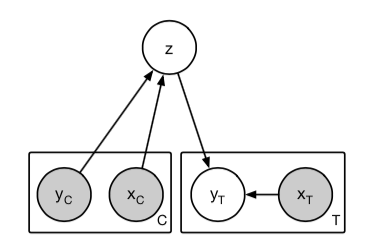
\includegraphics[width = 6cm]{graphicalmodel_NP.png}
  \caption{Graphical Model of Neural Processes~\cite{garnelo2018neural}. $x$ is the input data and $y$ is the output data corresponding to $y = f(x)$. $(x_{c},y_{c})$ are the context points which are observed and $C$ is the number of context points.$(x_{t},y_{t})$  are the target points and $T$  is the number of the target points. $x_{t}$ is not observed while $y_{t}$ is not observed. $z$ is the global latent variable.}
\end{figure}

The generative mechanism is shown in Figure 2 as continue lines: 
\begin{itemize}

\item First, an encoder $h$ from input space into representation space that takes in pairs of context values $(x_{c}, y_{c})$ and obtains a latent representation $r_{c} = h((x_{c}, y_{c}))$ for each of the pairs.

\item Second, an aggregator $a$ that summarises the vectors $r_c$ to obtain a single value $r$ (which has the same dimensionality as every $r_c$). This $r$ is used to parameterise the distribution of latent varibale $z$ i.e. $p(z|x_{1:C},y_{1:C}) = \mathcal{N}(\mu_z{r},\sigma_{z}^{2}(r))$. 

\item Finally, to obtain a prediction at a target $x_{t}$, we sample $z$ and concatenate this with $x_{t}$, and map $(z,x_{t})$ through a decoder $g$ to obtain a sample from the predictive distribution of $y_{t}$. 

\end{itemize}

\begin{figure}[h!]
  \centering
  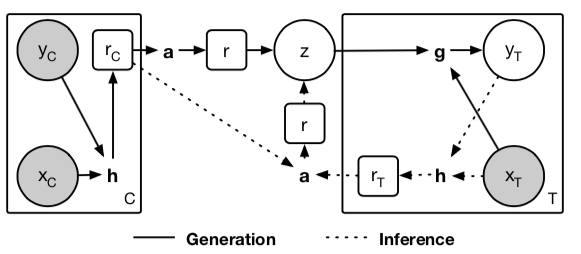
\includegraphics[width = 8cm]{computatioanaldiagram_NP.png}
  \caption{Computational Diagram of Neural Processes~\cite{garnelo2018neural}. Variables in circles correspond to the variables of the graphical model in Figure 1, variables in square boxes to intermediate representations of neural processes and unbound, bold letters to the following computation modules: $h$ - encoder. $a$ - aggregator and $g$ - decoder. $h$ and $g$ correspond to neural networks and $a$ to the mean function. The continue lines show the generative process and the dotted lines show the inference}
\end{figure}



Inference for the NP is carried out in the variational inference framework, shown in Figure 2 as dotted lines. Specifically, we introduce two approximate distributions:
\begin{itemize}
\item $q(z|\mbox{context})$ to approximate the conditional prior $q(z|\mbox{context})$.
\item $q(z|\mbox{context}, \mbox{target})$ to approximate the conditional prior $q(z|\mbox{context})$.
\end{itemize}
We use the same encoder $h$ to map both the context set and the target set to obtain the aggregated $r$ which in turn is mapped to $\mu_z$  and $\sigma^2_z$. These parametrise  the approximate posterior $q(z|\cdot) = \mathcal{N}(\mu_z,\sigma^2_z)$ 

The evidence lower bound(ELBO)
\begin{equation}
 \mbox{ELBO} = \mathbb{E}_{q(z|\mbox{context},\mbox{target})} \large[\sum_{t=1}^{T} \log p(y_{t}^{*}|z,x_{t}^{*}) + \log \frac{q(z|\mbox{context})}{q(z|\mbox{context},\mbox{target})}\large]
\end{equation}
The first term is the expected log-likelihood over the target set. The second term has a regularising effect - it is the negative KL divergence between q(z|\mbox{context}) and q(z|\mbox{context},\mbox{target}). 

Therefore, even the data is separated into context and target sets. The target set is directly used in training the NP model. This will allow the model to avoid overfitting and achieve better out-of-sample generalisation. In practice, we would repeatedly split our training data into randomly chosen context and target sets to obtain good generalisation. This split can be seen from the meta-learning viewpoint. Given $D$ data sets $d = 1,...,D$ has its own underlying function $f_{d}$ which has generated the values $y_{i} = f_d(x_{i})$, we might want to learn the posterior of every $f_{d}$ as well as generalise to a new data set $d^*$. The latter is especially useful when every data set has only a small number of observations. This information sharing is achieved by specifying that there exists a shared process which underlies all functions $f_{d}$. For example, in the context of $GPs$, one can assume that $f_d \sim \mathcal{GP}$ share kernel hyperparameters. Having learned the shared process, when given a new data set $d^{*}$, one can use the posterior over functions as a prior can carried out few-shot function regression. We would go through the procedure in the next parts using 1-D function regression task as an example.


\section{Results}
Here, we apply neural processes to a 1-D function regression task. The procedure is: 
\begin{itemize}
\item (1) Draw $f_d \sim GP(0,k(\theta))$ 
\item (2) Draw $x_{i} \sim \mathcal{U} (-2,2)$ 
\item (3) Define $y_{i} : = f_d(x_{i})$ 
\item (4) Divide pairs $(x_{i},y_{i})$ into context data $(x_{i},y_{i})_{C}$ and target data $(x_{i},y_{i})_{T}$. We would set the maximum context data points. Therefore in the simulation, the number of context data points would be a random value between three and maximum context data points. 
\item (5) Perform one optimization step. 
\item (6) Repeat from (1)
\end{itemize}

\begin{figure}[h!]
  \centering
  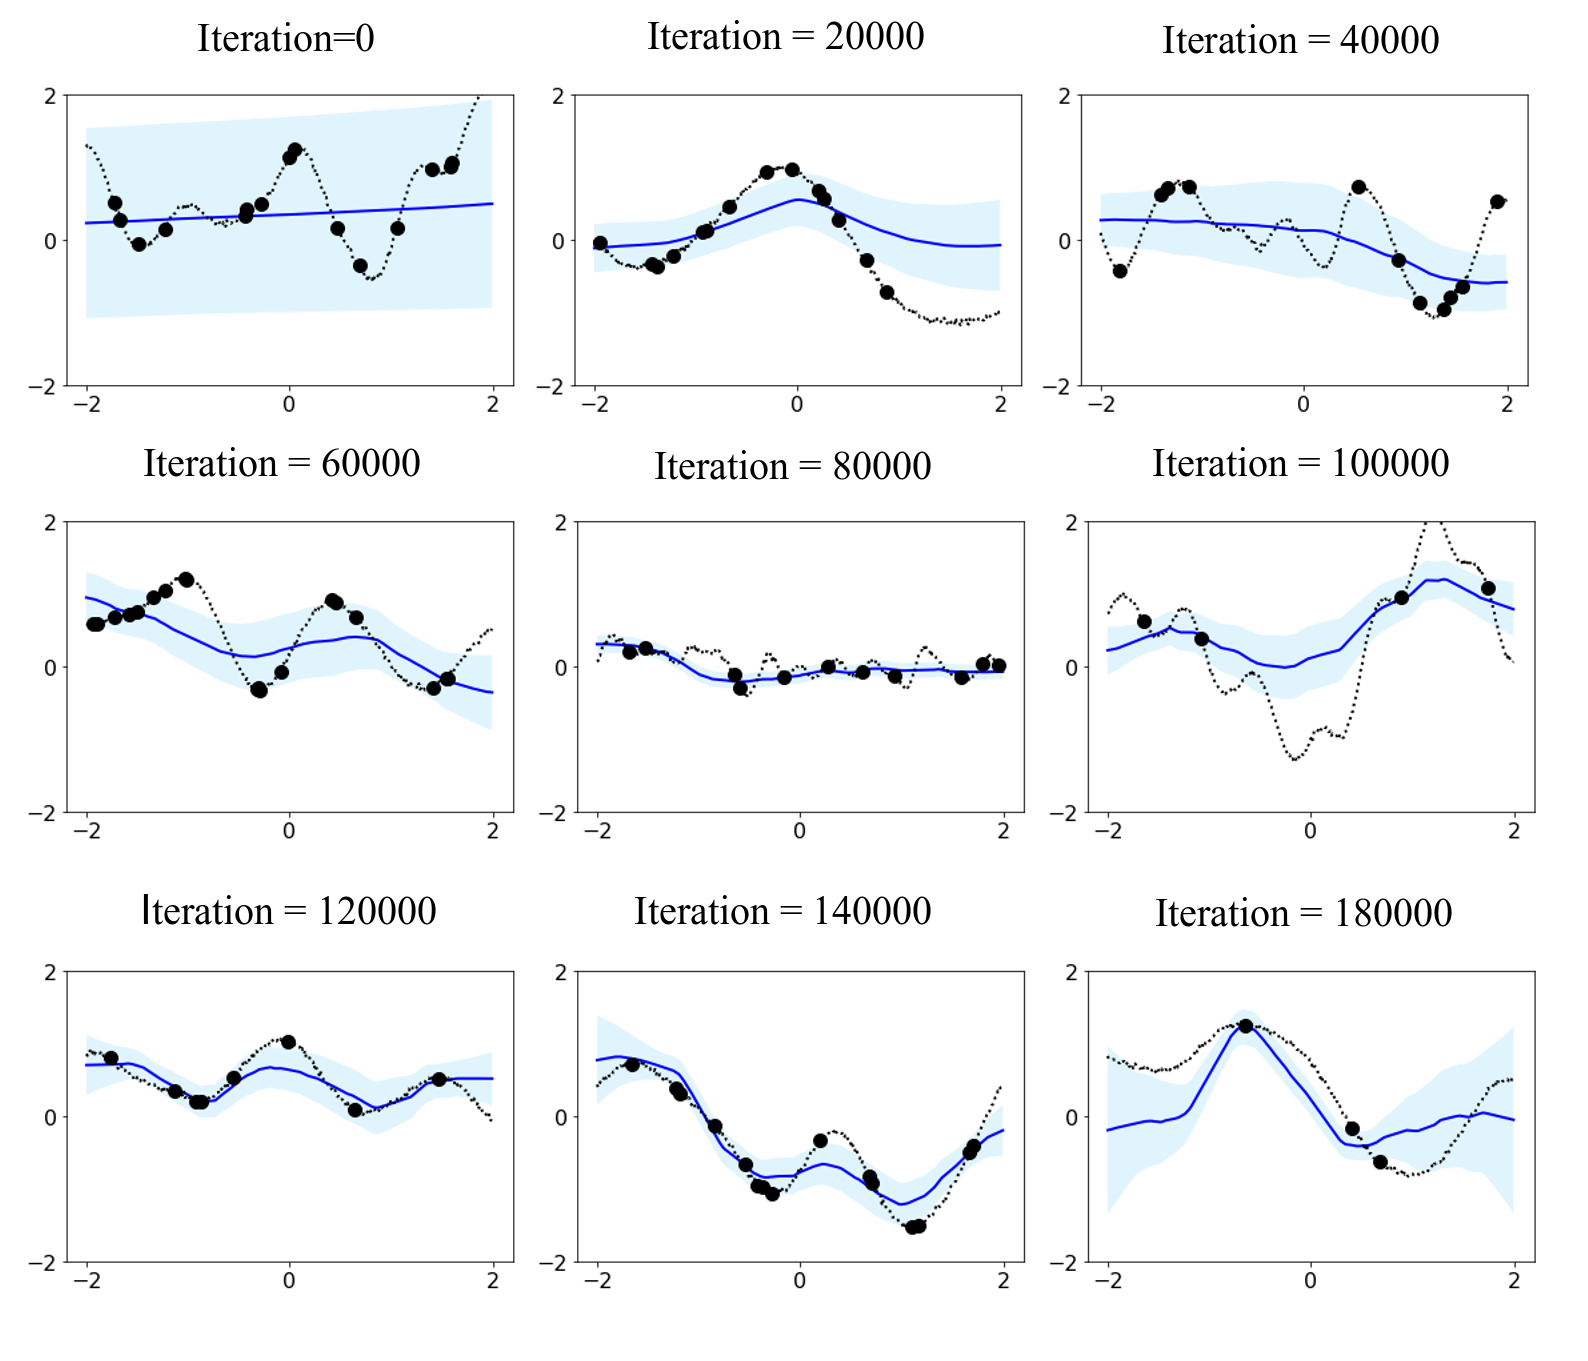
\includegraphics[width = 10cm]{NPS_1D_regression.png}
  \caption{1-D function regression using neural processes (maximum context data point is 20), and how the regression behaviors when the iteration increases. The black dots are context points $(x_c, y_c)$. The black dotted lines are the target points $(x_t, y_t)$. The blue continue lines show the predicted mean and the blue background shows the predicted variance for neural processes. The number of context data points is a random value between three and maximum context data points. Neural processes can represent distributions over functions. However, we also find that the context points are not always on the predicted mean line, which shows the underfitting and inaccurate predictions of neural processes.}
\end{figure}

In Figure 3, the maximum context data point is 20. Therefore, the number of context data point is a value between 3 and maximum context data points. Comparing the iteration = 120000, 140000, 180000 which the model is almost at equilibrium we find that as the number of context points increases, the sampled curves increasingly resemble the ground truth curve and the overall variance reduced. Also, we try setting different maximum context data points: 10, 20, 50. 

\begin{figure}[h!]
  \centering
  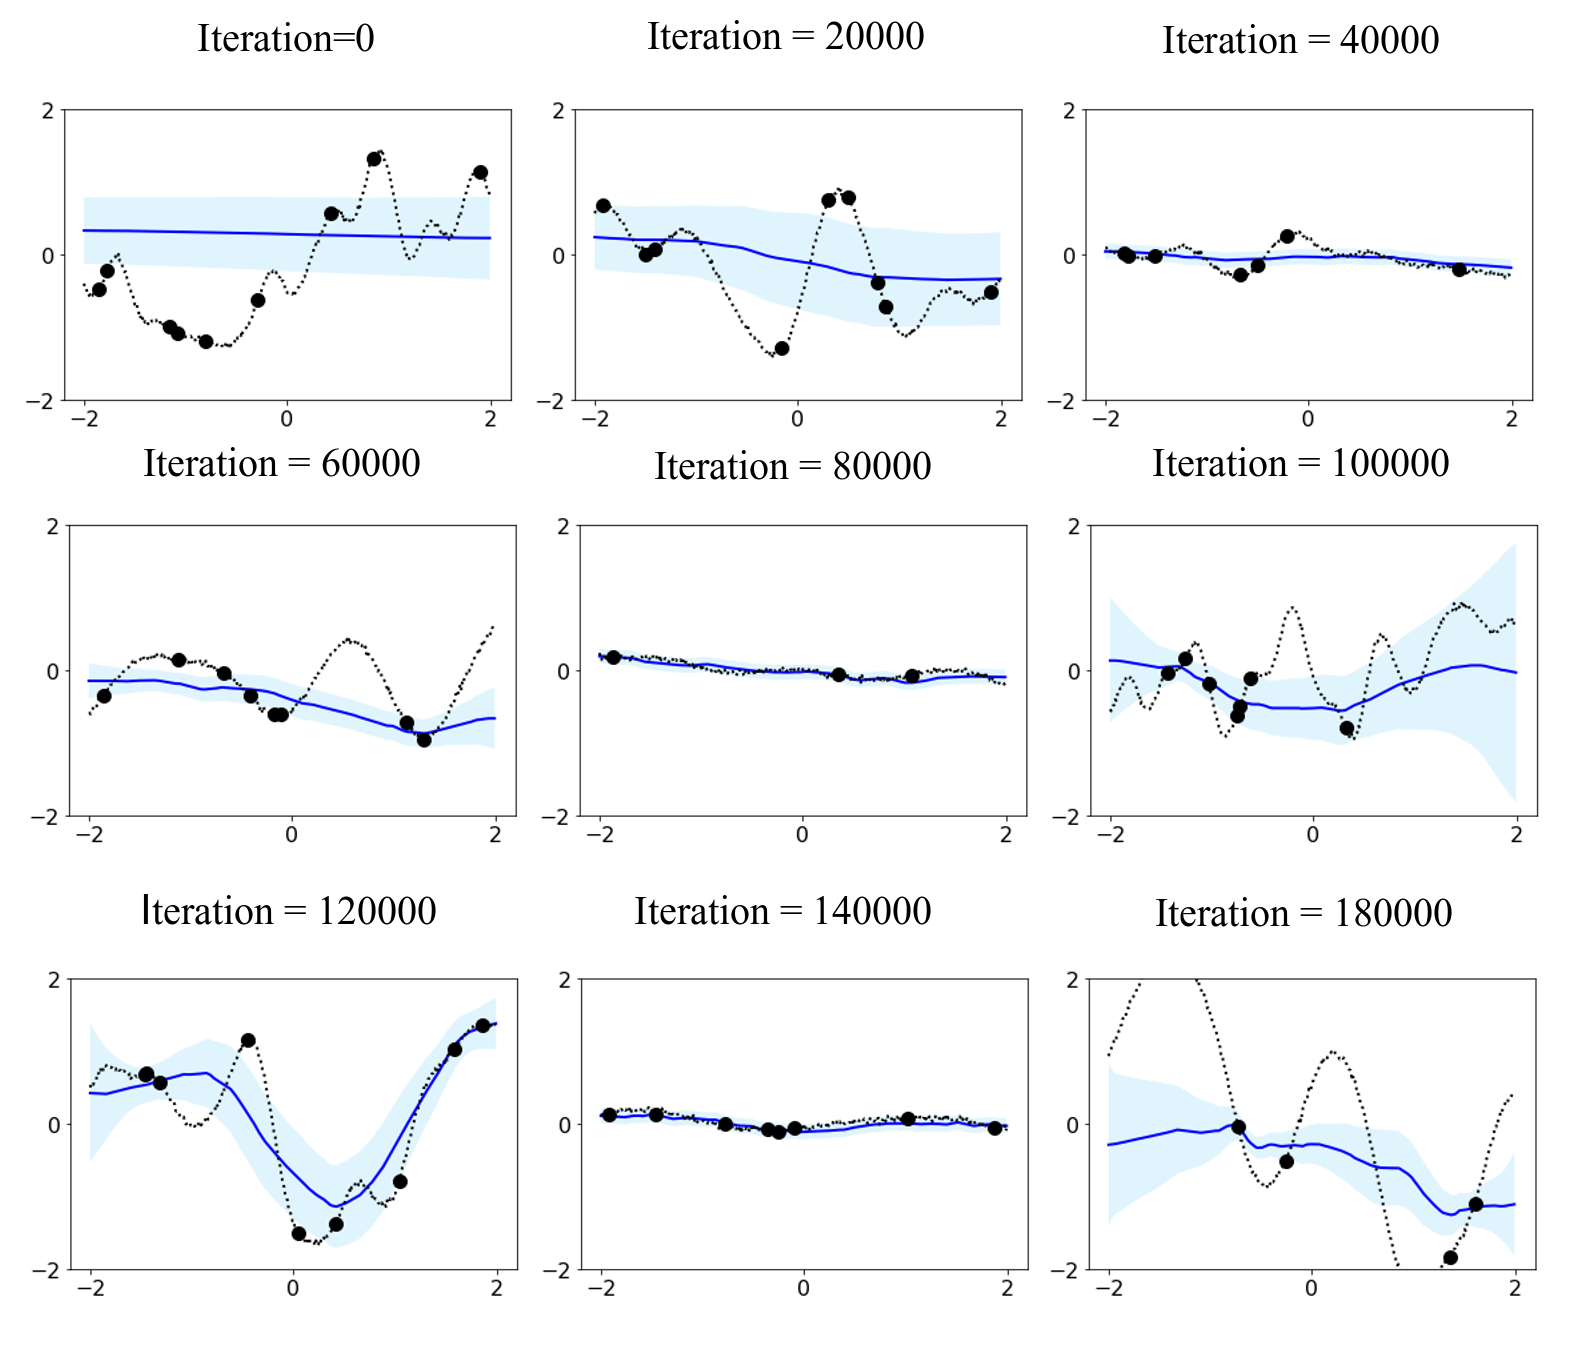
\includegraphics[width = 10cm]{NPS_1D_regression_cd10.png}
  \caption{1-D function regression using neural processes (maximum context data point is 10), and how the regression behaviors when the iteration increases.}
\end{figure}

\begin{figure}[h!]
  \centering
  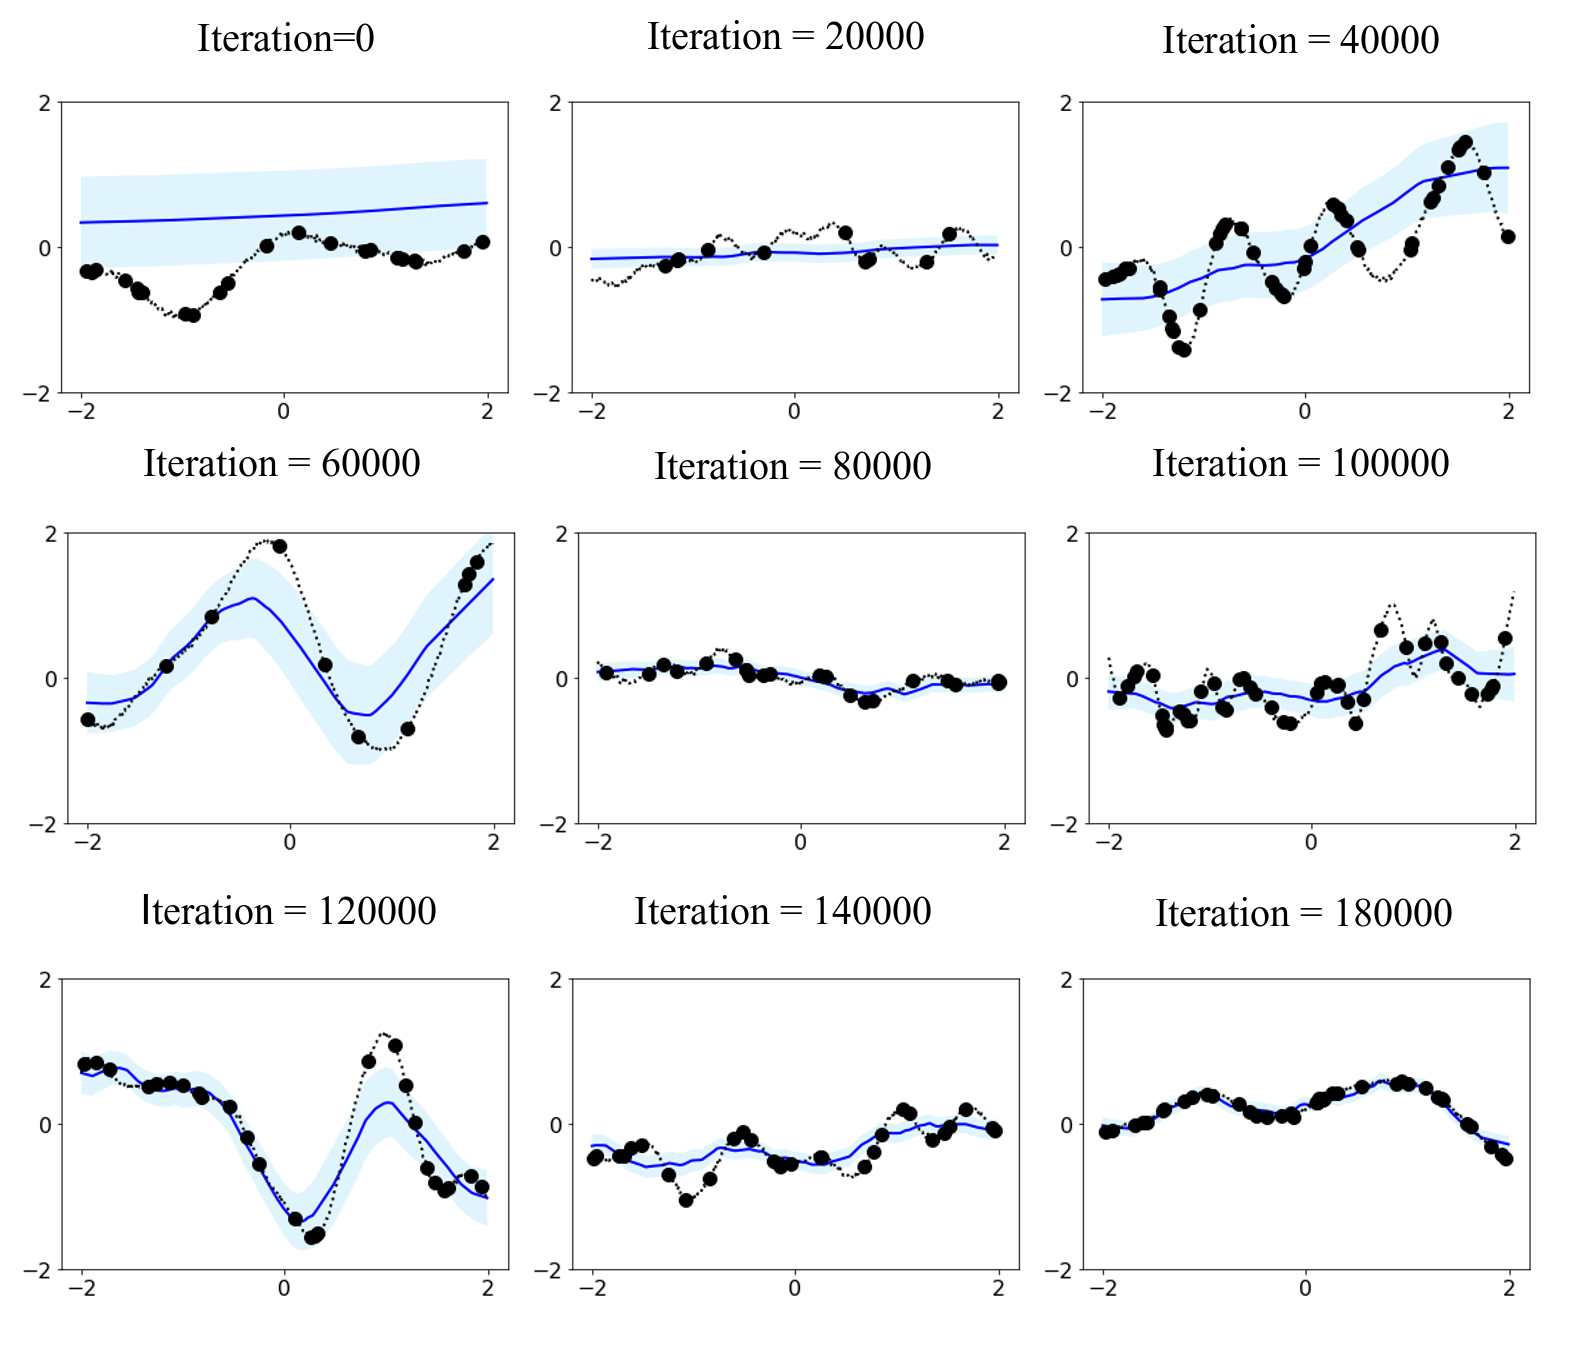
\includegraphics[width = 10cm]{NPS_1D_regression_cd50.png}
  \caption{1-D function regression using neural processes (maximum context data point is 50), and how the regression behaviors when the iteration increases.}
\end{figure}

Comparing the convergence in Figure 3 (maximum context data point is 20), Figure 4 (maximum context data point is 10) and Figure 5 (maximum context data point is 50), we find that the larger the maximum context data point, the faster the convergence.

\section{Discussions}
\label{discussions}
Neural processes can fit observed context data efficiently. Neural processes can learn a wide family of conditional distributions over functions. Neural processes can learn predictive distributions conditioned on context data sets with arbitrary size, which means that neural process can capture uncertainty. The maximum context data would effect the speed of convergence. In addition, instead of requiring a handcrafted kernel in Gaussian processes, neural processes learn an implicit measure from the data directly. Based on results of the 1-D regression shown in the Figure 3, 4, 5, neural processes do suffer a serious drawback of underfitting, giving inaccurate predictions for the context data. 

\begin{figure}[h!]
  \centering
  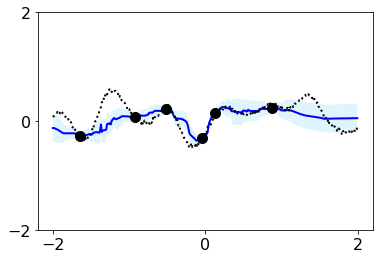
\includegraphics[width = 6cm]{ANP_1D_regression.png}
  \caption{1-D function regression using attentive neural processes at iterations = 180000. We find that the context points (black dots) are always on the predicted mean (blue line), which means attentive neural processes evidently improves the accuracy of predictions on the context points comprared to neural processes shown in Figure 3.}
\end{figure}

Deepmind recently address this issue by incorporating attention into NPs, which is called attentive neural processes~\cite{kim2019attentive} in a new paper (Here, we only briefly talk about the results of attentive neural processes since the length limit of the report). Attentive neural processes allow each input location to attend to the relevant context points for the prediction and this evidently improves the accuracy of predictions shown in Figure 6 compared to the Figure 3. But due to the attention, the complexity of attentive neural processes is raised from $\mathcal{O}(n+m)$ to $\mathcal{O}(n(n+m))$.

\section*{Acknowledgments}
I would like to thank Prof. Nicholas Zabaras for offering wonderful lectures. I would like to thank TA Dr. Souvik Chakraborty for giving assistants in homework and choosing the final project's topic. I would like to Xian Gao for insightful discussions. I would like to thank my advisor Prof. Jonathan K. Whitmer for supporting me to take this course for future research.

%\section*{References}

\bibliographystyle{abbrv}
\let\bibhang\relax
%\normalem
\bibliography{ref}
\end{document}
